% Chapter Template

\chapter{Swarm} % Main chapter title

\label{Chapter2} % Change X to a consecutive number; for referencing this chapter elsewhere, use \ref{ChapterX}

\lhead{Capítulo 2. \emph{Swarms}} % Change X to a consecutive number; this is for the header on each page - perhaps a shortened title

%----------------------------------------------------------------------------------------
%	SECTION 1
%----------------------------------------------------------------------------------------

\section{Comportamiento colectivo en la naturaleza}

\begin{figure}[htbp]
	\centering
		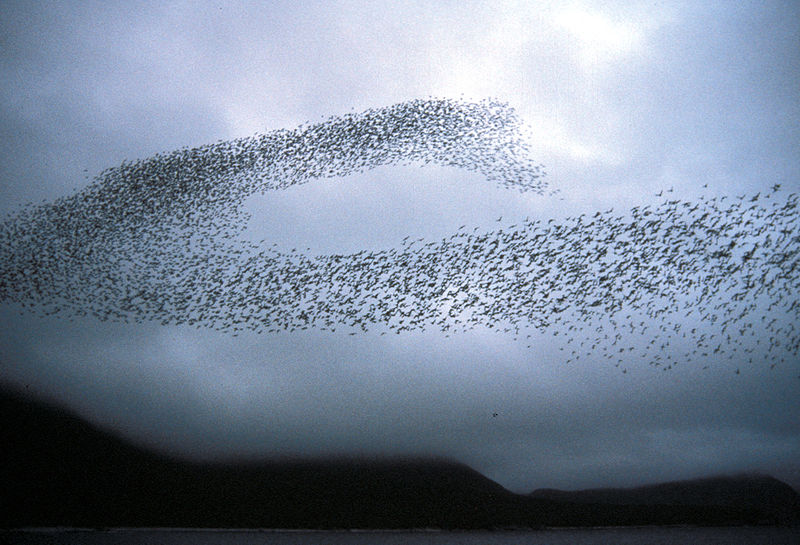
\includegraphics[width=0.8\textwidth]{./Figures/swarm.jpg}
		\rule{35em}{0.5pt}
	\caption[Bandada de auklets]{Bandada de auklets teniendo comportamiento de enjambre. Imagen tomada de Wikipedia.}
	\label{fig:Bandada}
\end{figure}

Existen casos de enjambres, los más típicos son las hormigas y abejas, pero los hay en peces, aves e incluso los mamíferos. Son sistemas donde nadie está a cargo y aún así ejecutan una tarea grupal. Las hormigas son un gran ejemplo. Al momento de construir su nido, no tienen un arquitecto o ingeniero estructural que esté dando órdenes, simplemente cada una sabe que tiene que hacer. No hay un director orquestando la construcción desde lo alto, en vez de esto lo que ocurre es un comportamiento emergente. También conocido como inteligencia de enjambre.

Otro tipo de comportamiento colectivo son las migraciones, desplazamientos periódicos que efectúan aves, peces, langostas y mamíferos de un hábitat a otro. Cada individuo activo en la migración sigue al grupo, los más pequeños como el plancton o anfibios aprovechan las corrientes de aire o agua, y las aves, más grandes, aprovechan los vientos y corrientes ascendentes. Hay diversas finalidades detrás de la migración, algunas especies lo hacen para escaparse de los crudos inviernos o secos veranos; mientras que otras, como las tortugas marinas, por una necesidad reproductiva emprenden un largo viaje de más de 10.000 millas, a lo largo de todo el Atlántico Norte.

Lograr que un enjambre de robots tenga un comportamiento emergente como el de las colonias de abejas es la piedra filosofal de los investigadores de esta área. Uno de los más destacados investigadores del área James McLurkin, experto en robótica del Massachusetts Institute of Technology (MIT); dice que para lograrlo es necesario un software que ejecute tareas individuales y     que de alguna forma se cumpla con una tarea grupal. He aquí una importante razón para desarrollar estudios sobre enjambres de robots, ya que aún no está claro cómo se coordina la naturaleza para llevar a cabo tales tareas.

%-----------------------------------
%	SECTION 2
%-----------------------------------
\section{Robots para construir un enjambre}

Diferentes laboratorios del mundo han tratado de construir robots que funcionen como enjambre con algún diseño que satisface sus propios requerimientos. Dependiendo de ellos varían en costo, tamaño y funcionalidad.

Algunos robots que pueden ser utilizados para hacer un Robot Swarm junto con las información técnica disponible, son listados en la sub secciones siguientes.

%-----------------------------------
%	SUBSECTION 1
%-----------------------------------
\subsection{Kilobot}
El proyecto Kilobot, ver figura \ref{fig:robots estudiados} a, es un sistema de bajo costo escalable para demostrar comportamientos colectivos. Actualmente existen varios grupos que están investigando algoritmos para enjambres de robots, por esto que diseñaron Kilobot que es un robot de bajo costo, accesible,  que permite hacer pruebas en cientos o miles de robots.

%-----------------------------------
%	SUBSECTION 2
%-----------------------------------
\subsection{Organismo Multibot}
S. Kornienko et al. \cite{5359578}, exploran el trabajo colaborativo en robots para un mejor rendimiento y mayor fiabilidad a nivel macroscópico. En este articulo demuestran sus últimos trabajos en sistemas colectivos y lo más sorprendente es que logran la agregación y desagregación autónoma para así obtener un organismo multibot. Este robot tiene la ventaja de tener un mecanismo que le permite unirse mecánicamente, pero también puede compartir energía, sensores y lógica con otros robots iguales para formar un organismo que es capaz de modificar su estructura y adaptarse al entorno auto-organizandose. En la figura \ref{fig:robots estudiados} b se puede ver una estructura formada por los robots.

%-----------------------------------
%	SUBSECTION 3
%-----------------------------------
\subsection{e-puck}
Uno de los robots más utilizados por los científicos en el mundo para estudios y publicaciones es el e-puck \cite{mondada2009puck}. Este robot es compacto, tiene forma de cilindro con un diámetro de 7 [cm] y para moverse hace uso de sus dos ruedas, dejándolo en la categoría de robot con desplazamiento diferencial. Originalmente fue diseñado para educar en el área de la micro ingeniería por Michael Bonani y Francesco Mondala en el laboratorio ASL del Profesor Roland Siegwart en Escuela Politécnica Federal de Lausana (EPFL) en Suiza. El e-puck es open hardware, software es de código abierto,  lo construyen y venden varias empresas. Para comunicarse con una computador incorporan un módulo Bluetooth conectado a uno de sus dos puertos serie. Existen varios tipos de accesorios, entre los que destacan un Zigbee para comunicaciones, un módulo con varias cámaras y LEDs RGB como sistema de comunicación visual. Su precio a la fecha en Gctronic es 912 USD. Para comprarlo hay que encargarlo desde Suiza.

%-----------------------------------
%	SUBSECTION 4
%-----------------------------------
\subsection{3pi Robot}
Pololu, la misma marca que tiene desarrollo de varios tipos de motores para robótica y PCB para controlarlos, diseño el 3pi Robot \cite{thurskyusing}. Es un robot bastante más económico que el e-puck, cuyo valor es 99.95USD ref. Sparkfun. También tiene dos ruedas para desplazarse de forma diferencial, 5 sensores de reflectancia, un LCD de 8x2 caracteres, un buzzer y tres botones para que el usuario pueda programarlos. Todos estos dispositivos están conectados a un microcontrolador ATmega328. Su velocidad es de 90 cm/s.

El 3pi fue diseñado especialmente como un robot seguidor de lineas y solucionar laberintos. Existen varios videos que muestran la asombrosa velocidad de estos robots para solucionar un laberinto. Se programa en C, pero como posee un microcontrolador ATmega es posible hacer uso del bootloader Arduino y programarlo con ese IDE. Usa 4 baterías AAA y trae 4 LEDs. No incorpora ningún tipo de comunicaciones inalámbrica. 


\begin{figure}[htbp]
	\centering
		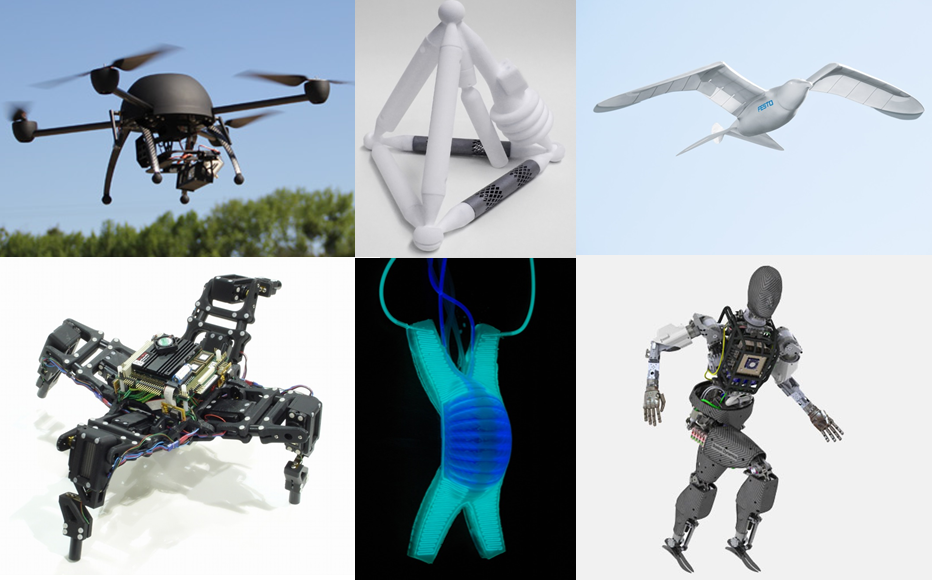
\includegraphics[width=\textwidth]{./Figures/robots.png}
		\rule{35em}{0.5pt} 
	\caption[Robots estudiados como alternativa para armar un enjambre de robots.]{\textbf{a.} Kilobot, el más simple de todos y pequeño. Imagen tomada de \cite{6224638}. \textbf{b.} Organismo Multibot, permite armar estructuras con los robots. Imagen tomada de \cite{5359578}. \textbf{c.} e-puck, robot altamente difundido en investigaciones, caro y complejo. Imagen tomada de \cite{mondada2009puck}. \textbf{d.} 3pi Robot, simple y económico pero no tiene comunicación inalámbrica. Imagen tomada de \cite{thurskyusing}}
	\label{fig:robots estudiados}
\end{figure}

En la Figura \ref{fig:Tabla robots} hay una tabla comparativa que resume las principales características de los robot: Kilobot\footnote{http://www.k-team.com/mobile-robotics-products/kilobot/specifications}, e-puck\footnote{http://www.gctronic.com/doc/index.php/E-Puck} y 3pi\footnote{http://www.pololu.com/catalog/product/975/specs}. Lamentablemente para el multibot no es mucha la información disponible.

\begin{figure}[htbp]
	\centering
		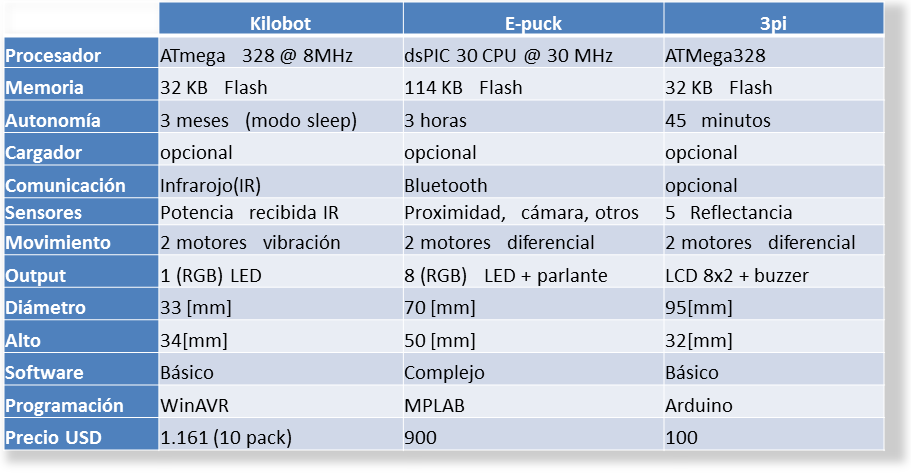
\includegraphics[width=1\textwidth]{./Figures/tabla_robots.png}
		\rule{35em}{0.5pt}
	\caption[Tabla comparativa robots]{En esta tabla se comparan las caracteristicas principipales de los robots: kilobot, e-puck y 3pi. No se incluyó el robot utilizado para el organismo multibot ya que no se comercializa.}
	\label{fig:Tabla robots}
\end{figure}

%-----------------------------------
%	SECTION 3
%-----------------------------------
\section{Necesidades de mercado}

De los robots estudiados destaca en sus prestaciones el e-puck, pero este tiene dos grandes problemas para ser usado por gente que no es especialista en robots. Uno es que tiene demasiado hardware, lo que tiende a confundir y aumentar costos. Dos, que para su comunicación inalámbrica hace uso de Bluetooth, protocolo que no soporta las redes Mesh para hacer de manera simple el control de muchos dispositivos en una red. Por otro lado el robot Kilobot es extremadamente simple, no permite mucha modificación ni control y el robot 3pi es algo grande en tamaño para trabajar en laboratorio con varios al mismo tiempo. Ninguno de los dos últimos tiene sistema de comunicación inalámbrica.

Hace falta un robot que no sobrepase los 200 USD, capaz de controlarse en forma inalámbrica, simple de construir y fácil de usar. Se requiere hacer uso de tecnologías como impresoras 3D y diseño Open Hardware - Open Source para formar el enjambre. Tener un diseño compatible con las impresoras 3D facilita enormemente la distribución del proyecto ya que cualquier persona con acceso a una impresora 3D puede replicar el robot. Y para hacer más simple el proceso de replica y fomentar las mejoras en el proyecto se requiere que tanto el hardware como el software sean Open, esto significa por ejemplo, que cualquier persona puede acceder al código fuente del robot, copiarlo, redistribuirlo y modificarlo para que se adapte a sus necesidades.

\begin{figure}[htbp]
	\centering
		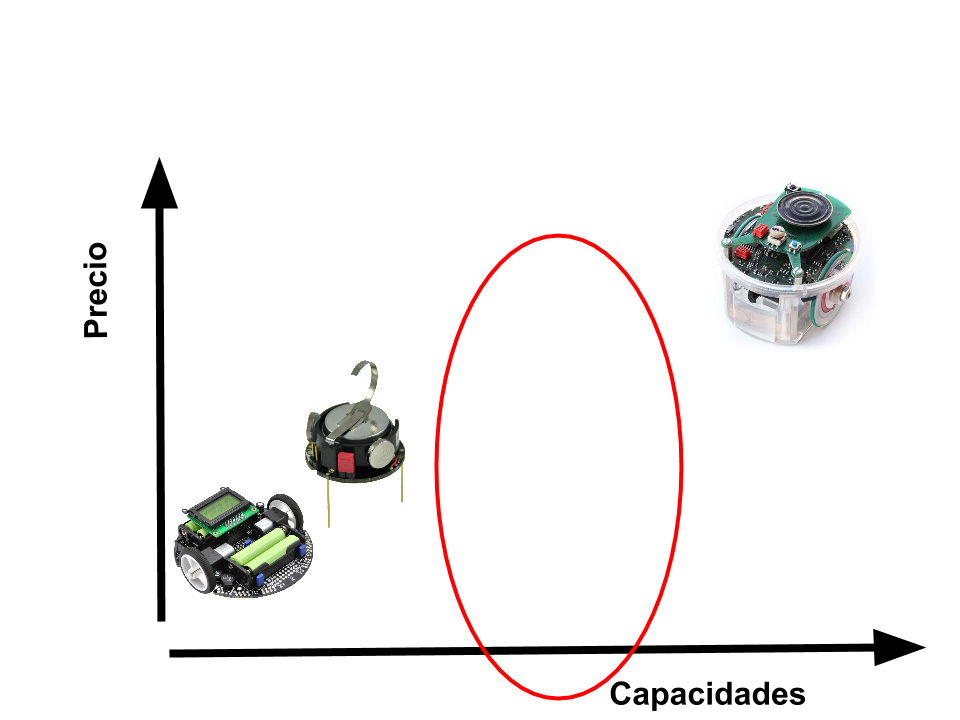
\includegraphics[width=0.8\textwidth]{./Figures/nicho.png}
		\rule{35em}{0.5pt}
	\caption[Nicho de mercado]{Nicho de mercado donde puede ingresar MODI}
	\label{fig:nicho}
\end{figure}


